

\section{Фотоны. Законы фотоэлектрического эффекта. Уравнения Эйнштейна. Внутренний фотоэффект. Фотоэлементы и их применения: фотоэлектронный умножитель(ФЭУ).}

\subsection{Фотоны}


Фотоны - кванты света, энергия которых определяется формулой

\begin{equation*}
    E = h\nu
\end{equation*}
\subsection{Фотоэффект}

Сущность явления состоит в том, что при освещении ультрафиолетовыми лучами отрицательно заряженного металлического тела оно теряет отрицательный заряд. При освещении такими же лучами положительно заряженного тела потери заряда не наблюдается. Более того, если тело не было заряжено, то при освещении оно заряжается положительно до потенциала в несколько вольт. После открытия электрона в 1897 г. Дж. Дж. Томсоном (1856—1940) опытами самого Томсона, а также Ленарда (1862—1947) вскоре был найден удельный заряд е/m для частиц, теряемых телами при освещении. Он оказался таким же, как и для частиц катодных лучей. Тем самым было доказано, что при освещении тела теряют электроны.
Явление вырывания электронов из вещества при освещении его светом получило название фотоэлектрического эффекта или, короче, \textit{фотоэффекта}.

\bigskip

Различают внешний и внутренний фотоэффект. При внешнем фотоэффекте электроны освобождаются светом из поверхностного слоя вещества и переходят в другую среду, в частности в вакуум. При внутреннем фотоэффекте оптически возбужденные электроны остаются внутри освещаемого тела, не нарушая электрическую нейтральность последнего. Для обоснования гипотезы фотонов основное значение имеет внешний фотоэффект, который преимущественно и рассматривается в этом параграфе. О внутреннем фотоэффекте и о его применениях будет сказано несколько слов в конце этого же параграфа.

Электроны, вырванные под действием света, называются фотоэлектронами. Фотоэлектрическими свойствами обладают как металлы, так и диэлектрики, а также полупроводники и электролиты, причем необходимым (но недостаточным) условием фотоэффекта является заметное поглощение используемого света в поверхностном слое освещаемого тела. Фотоэлектрический эффект вызывается не только ультрафиолетовыми лучами. Щелочные металлы — литий, натрий, калий, рубидий, цезий — весьма чувствительны к фотоэлектрическому действию и в видимой области спектра. А специальная обработка поверхностей этих и других металлов делает их способными испускать фотоэлектроны даже под действием инфракрасных лучей.


\begin{figure}[h!]
    \centering
    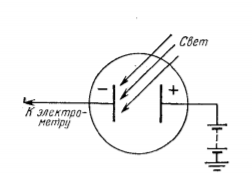
\includegraphics[scale=1.5]{phef.png}
    \label{fig:my_label}
\end{figure} 

На рисунке показана принципиальная схема экспериментальной установки для исследования фотоэффекта. Фотоэлектроны, вырванные при освещении из катода, увлекаются приложенным напряжением к аноду и замыкают цепь. По скорости зарядки электрометра (вместо электрометра можно взять чувствительный гальванометр) можно определить силу электрического тока в цепи, а с ней и количество фотоэлектронов, достигающих анода в единицу времени. Опыты подобного рода в ранних исследованиях производились в газах. Но их лучше производить в вакууме, так как газ только осложняет явления, происходящие в поверхностном слое металла.

\subsection{Внутренний фотоэффект}

Внутренний фотоэффект может происходить в полупроводниках и диэлектриках. Под действием света часть электронов из валентной энергетической зоны переходит в зону проводимости. Концентрация носителей тока внутри тела увеличивается — возникает фотопроводимость, т. е. повышение электрической проводимости тела под действием света. Перераспределение электронов по различным энергетическим состояниям может привести также к изменению внутреннего электрического поля в кристалле. Это ведет к появлению электродвижущей силы (фото-эдс) на границах двух различных полупроводников или полупроводника и металла при их осбещении. Около границы образуется переходный слой, пропускающий ток только в одном направлении, т. е. обладающий вентильными свойствами.


\subsection{Уравнение Эйнштейна}

Уравнение Эйнштейна описывает максимальную кинетическую энергию, которой может обладать вылетевший электрон:

\begin{equation*}
    \frac{m_ev^2_{max}}{2} = h\nu - A,
\end{equation*}
где $A$ - работа выхода, $m_e$ - масса покоя электрона.
\subsection{Фотоэлементы и их применения}

Фотоэффект (как внешний, так и внутренний) используется в фотоэлектронных приборах, получивших разнообразные применения в науке и технике (в телевидении, космической технике и т. д.). Нашли широкое применение фотоэлементы с внешним фотоэффектом, т. е. двухэлектродные приборы, в которых падающая на поверхность катода лучистая энергия при внешнем приложенном напряжении между электродами превращается в энергию электрического тока. Электрическое сопротивление полупроводников падает при освещении; это используется для устройства фотосопротивлений. Возникновение фото-эдс при освещении приконтактной области двух различных соприкасающихся полупроводников используется в фотодиодах для непосредственного превращения лучистой энергии в электрическую. 

\subsection{Фотоэлектронный умножитель}

Сивухин, том 3, $\S 103$
\begin{figure}[h!]
    \centering
    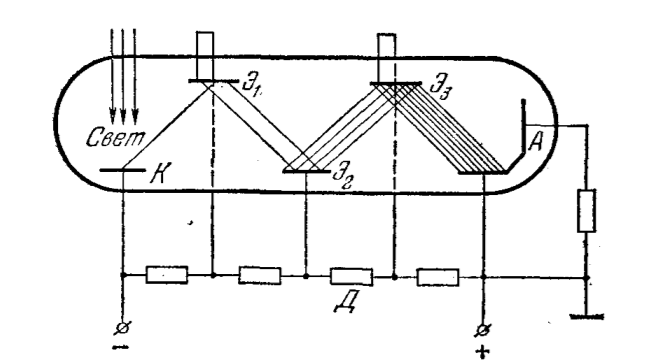
\includegraphics[scale=1]{feu.png}
    \label{fig:my_label}
\end{figure} 

\textit{Вторичная электронная эмиссия} - явление испускания вторичных электронов при бомбардировке пучком электронов поверхностей металлов, полупроводников или диэлектриков.

\textit{Фотоэлектронный умножитель} - прибор, основанный на вторичной фотоэлектронной эмиссии, предназначенный для усиления слабых электрических токов. Этот прибор представляет собой вакуумную трубку с катодом К и анодом А, между которыми расположено несколько электродов, эмиттирующих вторичные электроды. На эти электроды подается электрическое напряжение посредством делителей Д. Падающее электромагнитное излучение вырывает электроны с поверхности катода. Под действием электрического поля слабый электронный пучок ускоряется и направляется к эмиттеру Э$_1$, на котором происходит вторичная электронная эмиссия. Электроны с первого эмиттера направляются на второй эмиттер Э$_2$, где происходит вторичное усиление, и т.д. В результате получается усиленный во много раз фототок, который и снимается с анода А.

